\documentclass[12pt]{article} % use larger type; default would be 10pt

%packages
\usepackage[utf8]{inputenc} % set input encoding (not needed with XeLaTeX)
\usepackage{fancyhdr}
\usepackage{float}
\usepackage{geometry}
\usepackage{ulem}
\usepackage{soul}
\usepackage{color}
\usepackage{graphicx}
\usepackage{hyperref}
\usepackage{array}
\usepackage{caption}
\usepackage{titling}
\usepackage{enumerate} 
\usepackage[dvipsnames]{xcolor}
\usepackage{amsmath}
\usepackage{amssymb}
\usepackage[compact]{titlesec}


 %put box around figure captions
\makeatletter
\long\def\@makecaption#1#2{%
  \vskip\abovecaptionskip
  \sbox\@tempboxa{\fbox{#1: #2}}%
  \ifdim \wd\@tempboxa >\hsize
    \fbox{\parbox{\dimexpr\linewidth-2\fboxsep-2\fboxrule}{#1: #2}}\par
  \else
    \global \@minipagefalse
    \hb@xt@\hsize{\hfil\box\@tempboxa\hfil}%
  \fi
  \vskip\belowcaptionskip}
\makeatother

%reduce space between 
\titlespacing{\section}{0pt}{*1}{*0}
\titlespacing{\subsection}{0pt}{*1}{*0}
\titlespacing{\subsubsection}{0pt}{*0}{*0}


%no indent and modify distance between paragraphs
\setlength\parindent{0pt}
\setlength\parskip{12pt}

%set margins and line spacing
\geometry{margin=1in}
\linespread{1.2}
\geometry{letterpaper}

%math operators
\DeclareMathOperator{\E}{\mathbb{E}}

%set up header and page numbering
\pagestyle{fancy}
\lhead{CS 155 Set 4}
\rhead{Timothy Liu}
\pagenumbering{arabic}



\title{CS155 Set 4}
\author{Timothy Liu}

\begin{document}

\maketitle
\newpage
\section{Problem 1}

\subsection{Problem A}
\subsubsection{Problem i}
The first neural network has weights initialized to what appear to be random numbers between -0.5 and 0.5 while the second neural network has weights all initialized to zero. After 250 iterations, the first network has a test loss of 0.001 while the second network that has weights initialized to 0 has test loss of 0.508. The ReLu function is non-differentiable at 0 and has derivative of zero for values less than 0. If the neural network weights are initiated at 0, then back propagation won't have a gradient to go down because it's sitting at the discontinuity. This means initiating weights at 0 will leave it stuck and unable to improve.

\subsubsection{Problem ii}
The neural net with weights initialized to zero again have the same problem. Because the weights are 0, when fed into the neural net all of the neurons go to zero. After 400 iterations, the neural net has a test loss of 0.374, which is much larger than the loss from ReLu. This is because the gradient of the sigmoid far from 0 is very small, so the weights change by very small amounts.

\subsection{Problem B}
If the neural net is only trained on the negative examples, then the weights will be pushed to the regime where the output is negative and the ReLU is flat. The nonlinearity will always output a zero so even when the positive examples are input the nonlinearities will still output a zero.


\subsection{Problem C}

\subsubsection{i}
\begin{figure}[H]
	\makebox[\textwidth][c]{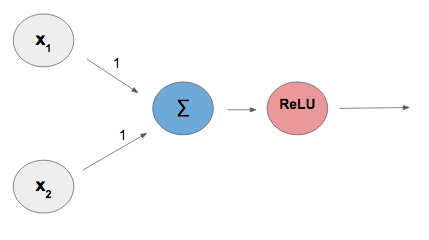
\includegraphics[width=4.2in]{1ci.png}}
	\vspace{-10mm}
	\caption{OR function. If either input is 1 then the output will be 1.}
\end{figure}


\subsubsection{ii}
\begin{figure}[H]
	\makebox[\textwidth][c]{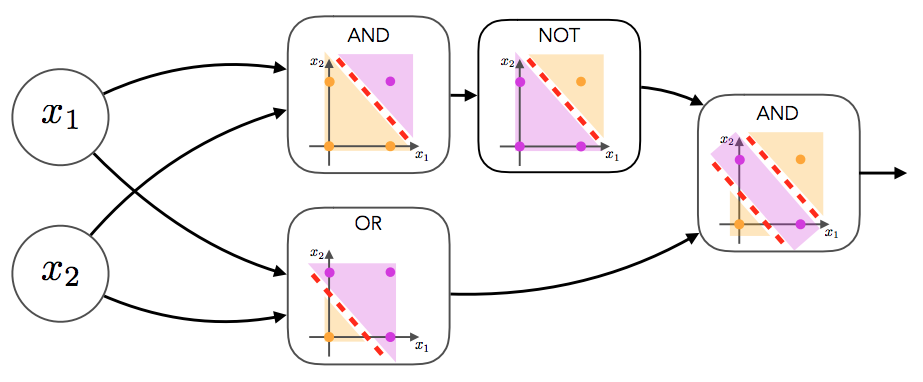
\includegraphics[width=4.2in]{1cii.png}}
	\vspace{-10mm}
	\caption{XOR function.}
\end{figure}

A minimum of 3 ReLU layers are needed. To make an XOR we need to AND together an inverted AND along with an OR. The AND, OR, and NOT operations each require one layer, and three must be stacked to create an exclusive OR.


\section{Problem 2}
\subsection{Problem A}
Tensorflow version: 1.5.0
Keras version: 2.1.3

\subsection{Problem B}
\subsubsection{i}
Each input example is a 2D 28 by 28 array. The elements in each array index are 8 bit grayscale value. 0 corresponds to black and 255 corresponds to white. There are 60,000 input examples, so the input array Xtrain has dimensions 60,000 by 28 by 28.

\subsubsection{ii}
The new shape of the training input is a 2D array with dimensions 60,000 by 784.

\subsection{Problem C}
The neural net has 100 hidden units organized in 2 layers with ReLU activation and no dropout. Batch size is set at the default of 32, run for 10 epochs, and using the Adam optimizer. The test accuracy is 0.9729.

\subsection{Problem D}
The neural net has 200 hidden units organized in 2 layers with ReLU activation and no dropout. Batch size is set at the default of 32, run for 10 epochs, and using the Adam optimizer. The test accuracy is 0.9808.

\subsection{Problem E}
The neural net has 1000 hidden units organized in 4 layers with ReLU activation and no dropout. Batch size is of 1024, run for 30 epochs, and using the Adam optimizer. The test accuracy is 0.9833.


\section{Problem 3}

\subsection{Problem A}

One benefit of zero-padding is that the result has the same dimensions and the same size as the original. You are neither upsampling nor downsampling. The disadvantage is that the image effectively has a black border around the edge, which may affect the results and disrupt the training.

\subsection{Problem B}

\subsubsection{i}
The number of weights is the size of the filter 5 x 5 x 3 + 1 multiplied by the 8 filters. This is 608 weights.

\subsection{ii}
The output tensor is 30x30x8 because since there is no zero-padding and the stride is 1, we have a little downsampling. The depth is the same as the number of filters.

\subsection{Problem C}
\subsubsection{i}

$$
\begin{bmatrix}
    1 & 0.5  \\
    0.5 & 0.25  \\
\end{bmatrix}
,
\begin{bmatrix}
    0.5 & 1  \\
    0.25 & 0.5  \\
\end{bmatrix}
,
\begin{bmatrix}
    0.25 & 0.5  \\
    0.5 & 1  \\
\end{bmatrix}
,
\begin{bmatrix}
    0.5 & 0.25  \\
    1 & 0.5  \\
\end{bmatrix}
$$

\subsubsection{ii}
$$
\begin{bmatrix}
    1 & 1  \\
    1 & 1  \\
\end{bmatrix}
,
\begin{bmatrix}
    1 & 1  \\
    1 & 1  \\
\end{bmatrix}
,
\begin{bmatrix}
    1 & 1  \\
    1 & 1  \\
\end{bmatrix}
,
\begin{bmatrix}
    1 & 1  \\
    1 & 1  \\
\end{bmatrix}
$$
\subsubsection{iii}
Pooling is advantageous because averaging several pixels together will smooth the image out and reduce noise. This may also reduce overfitting.

\subsection{Problem D}

\begin{figure}[H]
	\makebox[\textwidth][c]{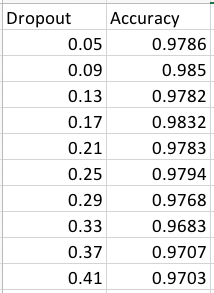
\includegraphics[width=2.5in]{drop_table.png}}
	\vspace{-10mm}
	\caption{Test accuracy with varying dropout rates.}
\end{figure}


\begin{figure}[H]
	\makebox[\textwidth][c]{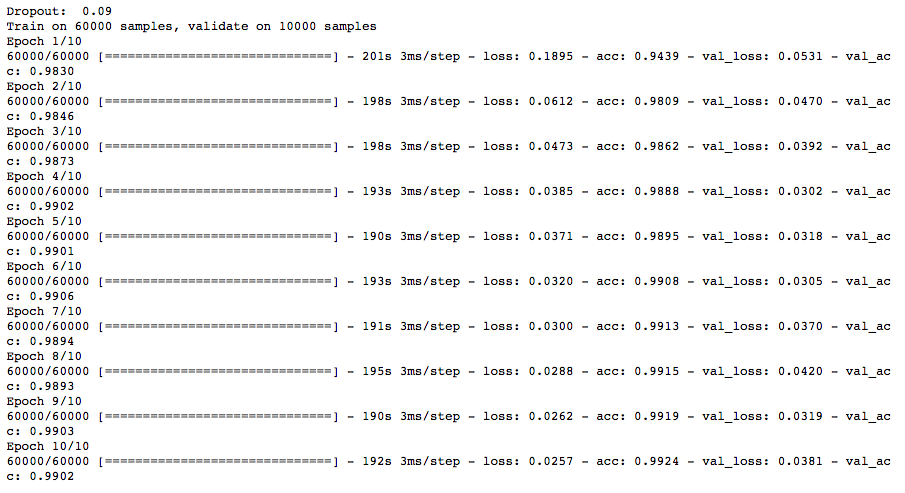
\includegraphics[width=6in]{final_model.png}}
	\vspace{-10mm}
	\caption{The final test accuracy after 10 epochs is 0.9902}
\end{figure}

\begin{figure}[H]
	\makebox[\textwidth][c]{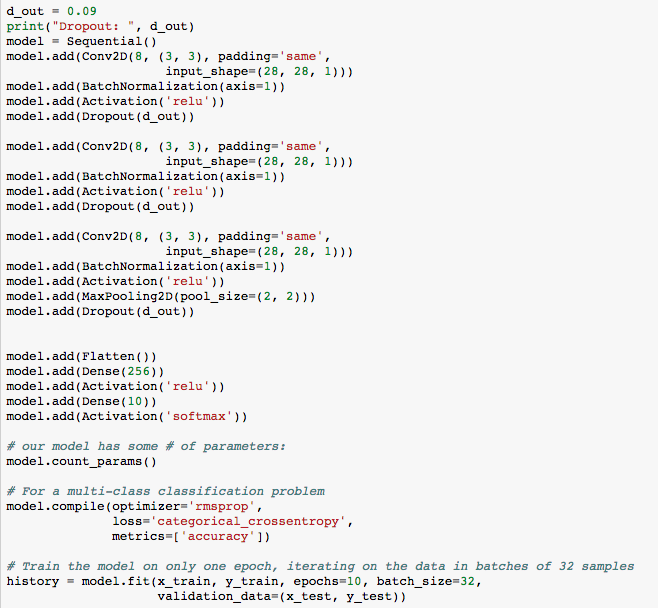
\includegraphics[width=6in]{final_model_code.png}}
	\vspace{-10mm}
	\caption{Code for final model.}
\end{figure}

The most accurate model layered several convolutional networks with MaxPooling towards the end. Greater max pooling was found to damage the accuracy. The final dense layer was increased to 256 units, which helped to boost performance. A fairly low amount of dropout combined with batch normalization also improved accuracy.

A problem with this type of optimization is that there are too many variables to optimize. Different variables may also affect each other, so for example a different amount of dropout may be more appropriate for a different number of convolution layers.










\end{document}
